\documentclass[11pt]{article}
\usepackage[letterpaper,margin=1in]{geometry}
\usepackage{amsmath,amssymb}
\usepackage{graphicx}
\usepackage{booktabs}
\usepackage{siunitx}
\usepackage{caption}
\usepackage[hidelinks]{hyperref}
\usepackage{enumitem}
\usepackage[expansion=false]{microtype}
\usepackage{titlesec}
\titlespacing*{\section}{0pt}{1.6ex plus .5ex}{0.8ex}
\titlespacing*{\subsection}{0pt}{1.2ex plus .4ex}{0.5ex}
\setlength{\textfloatsep}{10pt plus 2pt}
\setlength{\floatsep}{8pt plus 2pt}
\captionsetup{font=small,labelfont=bf}
\setlist{nosep,leftmargin=1.4em}
\graphicspath{{figures/}}
% AUTO-GENERATED by scripts/make_figures.py - do not edit by hand
\newcommand{\PropSource}{the reference values of Table~\ref{tab:params} (CoolProp run pending)}
\newcommand{\FLeo}{0.331}
\newcommand{\qLeo}{219}
\newcommand{\TsLeo}{259}
\newcommand{\qDeep}{109}
\newcommand{\TsDeep}{217}
\newcommand{\qMars}{47}
\newcommand{\TsMars}{176}
\newcommand{\Vbase}{71.2}
\newcommand{\Abase}{88.0}
\newcommand{\Rwall}{2.3\times10^{-6}}
\newcommand{\Rblanket}{3.16}
\newcommand{\WallRatio}{7.2\times10^{-7}}
\newcommand{\PhiH}{184}
\newcommand{\PhiO}{11.6}
\newcommand{\PhiM}{8.4}
\newcommand{\ArH}{44.7}
\newcommand{\ArO}{3.1}
\newcommand{\ArM}{2.3}
\newcommand{\tsH}{57}
\newcommand{\tsO}{1.6}
\newcommand{\tsM}{2.7}
\newcommand{\mzH}{256}
\newcommand{\mzO}{53}
\newcommand{\nzH}{60}
\newcommand{\QzH}{13.8}
\newcommand{\StrutShareH}{9}
\newcommand{\tsHsmall}{70}
\newcommand{\tsHbig}{48}
\newcommand{\tsOsmall}{2.2}
\newcommand{\tsObig}{1.4}
\newcommand{\tsMsmall}{3.3}
\newcommand{\tsMbig}{2.4}
\newcommand{\EnvSpread}{12}
\newcommand{\QholdH}{12.0}
\newcommand{\mliqH}{4{,}537}
\newcommand{\dTH}{5.2}
\newcommand{\thomH}{221}
\newcommand{\tcondH}{18}
\newcommand{\fcondH}{0.084}
\newcommand{\tcvH}{57.2}
\newcommand{\tcsH}{57.4}
\newcommand{\tccH}{76.8}
\newcommand{\tchH}{409}
\newcommand{\QholdO}{54.3}
\newcommand{\mliqO}{73{,}125}
\newcommand{\dTO}{12.2}
\newcommand{\thomO}{324}
\newcommand{\tcondO}{21}
\newcommand{\fcondO}{0.065}
\newcommand{\tcvO}{1.6}
\newcommand{\tcsO}{2.21}
\newcommand{\tccO}{61.7}
\newcommand{\tchO}{943}


\newcommand{\Qd}{\dot Q}
\newcommand{\md}{\dot m}

\title{\textbf{CryoSand: An Open Trade-Space Sandbox for\\In-Space Cryogenic Propellant Storage}\\[4pt]
\large First Written Report (Progress Report)}
\author{Vaishanth Srinivasan\\ M.S.\ Aerospace Engineering, San Jos\'e State University\\
Advisor: \textit{[name]}}
\date{September 25, 2026}

\begin{document}
\maketitle
\vspace{-1.5em}

\begin{abstract}
\noindent
CryoSand is an open tool for the in-space cryogenic storage trade: when does it pay to refrigerate a
propellant tank instead of only insulating it? This report covers the first month of the project. The
physics stack (layers L0--L5) has been specified, and build steps 1--7 are implemented, with 54 automated
tests passing (analytic limits plus CoolProp-backed closure tests). A first trade has been run with CoolProp
properties throughout. Five findings stand out.
(i)~The optimal cryocooler lift is always either zero or the full heat leak, never in between.
(ii)~For a vented tank with constant specific masses, the crossover duration has the closed form
$t^*=h_{fg}\,\mu_\text{act}$ and does not depend on insulation, tank size or environment.
(iii)~With the Strobridge cooler-mass correlation, a baseline LEO tank gives $t^*\approx\tsH$~days for LH$_2$
and $\approx\tsO$~days for LO$_2$. This is the same order as the published LEO estimates of $\sim$64 and $\sim$5~days.
(iv)~The textbook surface-layer closure ($\dot T_i=\Qd/m_\text{surf}c_p$) violates the ordering the bounding
argument needs: at 90\% fill it stores \emph{more} energy than the fully mixed tank. It was replaced by an
exact two-zone form whose ordering and collapse are now verified for three propellants and four fill levels.
(v)~Closing the tank shifts the crossover by roughly the hold time. With the exact bounds, the LH$_2$
crossover spans $\tcvH$ to $\tchH$~days depending on the ullage closure, and $\tcvO$ to $\tchO$~days for LO$_2$.
So the well-mixed assumption can move the crossover, not just the vent schedule.
\end{abstract}

%=====================================================================
\section{Problem and objectives}
A propellant tank in orbit holds liquid at 20--112~K behind an outer surface at roughly 180--260~K, so heat always leaks in.
Each watt that reaches the liquid evaporates it at $\md=\Qd/h_{fg}$ (for LH$_2$, 1~W boils off
$\approx$0.19~kg/day). A designer can spend mass on insulation and accept the boil-off, or on a cryocooler
plus its power system and radiator to remove the heat. The mission duration at which the second option
becomes lighter is the \emph{passive/active crossover} $t^*$. No open tool maps it; the fast storage codes
that could are licensed~\cite{zumbo}.

The project has two objectives:
\textbf{(E) engineering:} publish a map of $t^*$ across propellant, tank scale, environment and duration;
\textbf{(R) research:} determine whether the near-universal \emph{well-mixed ullage} assumption moves $t^*$
or only changes the vent schedule. Objective~R is answered by a \emph{bounding argument}. Two analytic
closures bracket the real pressure rise, and both are carried through the full trade. The spring CFD
campaign then refines where real tanks sit between the bounds, but the result does not depend on it.

%=====================================================================
\section{Physical model}
The model follows each watt from the Sun to the liquid in six independently testable layers (SI throughout;
fluid properties only from CoolProp~\cite{coolprop}).

\textbf{L0 Environment.} The outer surface absorbs sunlight, Earth albedo and Earth IR, and radiates to a
4~K sink. Averaged over a sphere's area,
\begin{equation}
q_\text{abs}=\alpha\left(\tfrac14 G_\odot + F_E\,a\,G_\odot\right)+\varepsilon F_E G_\text{IR},\qquad
\varepsilon\sigma\left(T_s^4-T_\text{sink}^4\right)=q_\text{abs},
\end{equation}
where $F_E=\tfrac12\left[1-\sqrt{1-(R_E/(R_E+h))^2}\right]$ is the sphere-to-Earth view factor. The inward
heat leak is less than 1\% of $q_\text{abs}$, so the outer-surface temperature $T_s$ is set by radiative equilibrium.

\textbf{L1 Insulation.} The multilayer-insulation (MLI) blankets are resistances in series. Struts and
plumbing bypass the blankets, so they form a \emph{parallel} conductance:
\begin{equation}
\Qd_\text{leak}=\frac{T_s-T_\text{sat}}{\sum_i t_i/(k_{\text{eff},i}A)+R_\text{wall}}
+G_\text{strut}\,(T_s-T_\text{sat}),\qquad
G_\text{strut}=\frac{A_s}{L_s}\,\bar k,\;\;\bar k=\frac{1}{\Delta T}\!\int k\,dT .
\end{equation}
The effective conductivity $k_\text{eff}$ lumps together radiation, spacer conduction and residual-gas
conduction. It is held constant at this fidelity.

\textbf{L2 Wall.} Fourier conduction $\nabla\!\cdot(k\nabla T)=0$ is solved by the Summer-2026 finite-difference
solver, which uses harmonic-mean face conductivities $k_f=2k_Pk_N/(k_P+k_N)$. At this stage it enters the
network as its 1-D limit, $R_\text{wall}=t/(kA)$.

\textbf{L3 Ullage and liquid.} Three closures, all first-class:
\begin{align}
\text{vented:}\quad & \md=\Qd_\text{net}/h_{fg},\\
\text{homogeneous (slow bound):}\quad & \dot u=\Qd_\text{net}/m,\;\; \rho=m/V,\;\; P=P(\rho,u),\\
\text{surface (fast bound):}\quad & \dot u_w=\Qd_\text{net}/m_w,\;\; \rho_w=m_w/V_w,\;\; P=P(\rho_w,u_w).
\end{align}
The homogeneous closure is the fully mixed tank, which gives the slowest possible pressure rise. The surface
closure puts all incoming energy into a \emph{warm zone}: an interface layer of liquid mass $m_\text{surf}$
together with the ullage vapour ($m_w=m_\text{surf}+m_v$). The rest of the liquid stays at its initial state
and occupies a fixed volume, so $V_w=V-(m_l-m_\text{surf})/\rho_l$. While the warm zone is two-phase, its
pressure is the saturation pressure of the interface, which gives the fast rise seen in stratified tanks.
Because the warm zone is a subset of the tank, $m_\text{surf}\to m_l$ recovers the homogeneous bound exactly.
The textbook form $\dot T_i=\Qd_\text{net}/(m_\text{surf}c_p)$ was used first and dropped (\S5).
$m_\text{surf}/m_l$ is swept. With $\Qd_\text{net}$ constant, each closure is summarised by the energy $E_\text{store}$ it can absorb
before reaching the vent pressure, which gives the hold time $t_\text{hold}=E_\text{store}/\Qd_\text{net}$.

\textbf{L4 Cooling.} The Carnot coefficient of performance is $\text{COP}_C=T_c/(T_h-T_c)$. The specific
power is $\phi=W_\text{in}/\Qd_\text{lift}=1/(\eta\,\text{COP}_C)$, where $\eta$ is the fraction of Carnot
achieved. The radiator rejects $\Qd_\text{lift}+W_\text{in}$, not $\Qd_\text{lift}$ alone:
$A_\text{rad}=\Qd_\text{lift}(1+\phi)/[\varepsilon\sigma(T_r^4-T_\text{sink}^4)]$. Cooler mass follows the
Strobridge correlation as scaled in~\cite{plachta2003},
$m_\text{cool}=0.2\,\Qd^{0.7}[(T_h-T_c)/T_c]^{1.45}$.

\textbf{L5 Closure.} $m_\text{pen}=m_\text{ins}+m_\text{cool}+m_\text{pow}+m_\text{rad}+m_\text{lost}$.
The crossover is the duration at which the minimum of $m_\text{pen}$ over the design space switches from
passive to active.

%=====================================================================
\section{Implementation status}
The code is in Python and follows three conventions: pure physics functions, frozen dataclasses for state,
and a single CoolProp property wrapper. Physics functions receive property values as arguments, so every
analytic limit can be tested without a property library. Table~\ref{tab:status} lists the build order.

\begin{table}[!htb]
\centering\small
\caption{Build order and status. All listed tests run under \texttt{pytest} with CoolProp installed.}
\label{tab:status}
\begin{tabular}{@{}llp{9.4cm}@{}}
\toprule
Step & Module & Status / verification\\
\midrule
1--2 & core, \texttt{network} & Done. Series chain matches the hand sum to $10^{-10}$; $k_f(2,6)=3$ exactly.\\
3 & L0, L1 & Done. View-factor limits $\{\tfrac12,0\}$; blankets scale as $1/n$; struts verified to be parallel.\\
4--5 & L4, L5, L3 vented & Done. Carnot limits (14, 2.33~W/W); radiator rejects lift plus work; ZBO balance; zero leak gives exactly zero boil-off.\\
6 & \texttt{model} (steady) & Done. First end-to-end run; brute-force optimum reproduces analytic $t^*$ (\S\ref{sec:trade}).\\
7 & L3 closed bounds & Done. Ordering holds at every $m_\text{surf}$ for 3 propellants $\times$ 4 fills; collapse exact to $10^{-10}$; energy closes to 0.5\%; liquid-full guard.\\
8 & L2 port & 1-D form and cylinder$\to$plane limit done; 2-D port pending.\\
9--10 & \texttt{trade}, app & First crossover sweep done (Fig.~\ref{fig:map}); Streamlit interface not started.\\
\bottomrule
\end{tabular}
\end{table}

%=====================================================================
\section{Preliminary results}
\textbf{Baseline:} a cylinder with hemispherical ends, $r=2$~m, cylindrical length $3$~m
($V=\Vbase$~m$^3$, $A=\Abase$~m$^2$), 90\% fill at 1~atm. The insulation design unit is a 10-layer MLI
sub-blanket. Saturated properties are \PropSource. All specific masses are the provisional register values of
Table~\ref{tab:params}; the numbers below show the structure of the trade and are not final predictions.

\subsection{Environment, heat leak and wall}
The absorbed flux (with $\alpha/\varepsilon=0.32/0.86$) and the resulting surface temperature are
$\qLeo$~W/m$^2$ and $\TsLeo$~K in LEO at 400~km ($F_E=\FLeo$), $\qDeep$~W/m$^2$ and $\TsDeep$~K in deep space
at 1~AU, and $\qMars$~W/m$^2$ and $\TsMars$~K in Mars transfer. The wall resistance is
$R_\text{wall}=\Rwall$~K/W, or $\WallRatio$ of a single 10-layer sub-blanket ($\Rblanket$~K/W), even with a
pessimistic $k=10$~W/m$\cdot$K. It is \emph{computed} to be negligible, not assumed so. At the LH$_2$ ZBO
optimum ($\nzH$ layers, $\Qd_\text{leak}=\QzH$~W), the struts carry $\approx\StrutShareH$\% of the leak with the
current placeholder conductance.

\subsection{The cooler asymmetry}
Figure~\ref{fig:cooler} shows the thermodynamic core of the trade. At the assumed fractions of Carnot, lifting
1~W costs $\PhiH$~W of electrical power at 20~K but only $\PhiO$~W at 90~K and $\PhiM$~W at 112~K. Every
100~W lifted from LH$_2$ needs $\ArH$~m$^2$ of 300~K radiator, compared with $\ArO$~m$^2$ for LO$_2$.

\begin{figure}[!htb]
\centering
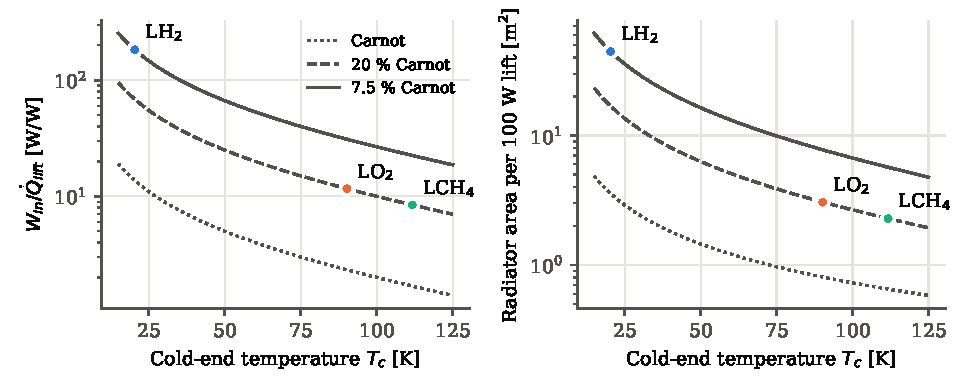
\includegraphics[width=0.8\linewidth]{fig1_cooler_asymmetry.pdf}
\vspace{-1.6em}
\caption{Specific power (left) and radiator area per 100~W of lift (right) against cold-end temperature, for
$T_h=T_r=300$~K and $\varepsilon_r=0.9$. Markers show each propellant at its assumed fraction of Carnot.}
\label{fig:cooler}
\end{figure}

\subsection{Structure of the trade and the vented crossover}\label{sec:trade}
\emph{End-point optimality.} For a fixed insulation choice, $m_\text{pen}(\Qd_\text{lift})$ is the sum of
terms that are linear in $\Qd_\text{lift}$ (power, radiator, and the boil-off of the uncovered leak) and
the concave cooler mass $\propto\Qd_\text{lift}^{0.7}$. A concave function on an interval has its minimum at
an end point. So the best design is always either fully passive ($\Qd_\text{lift}=0$) or full ZBO
($\Qd_\text{lift}=\Qd_\text{leak}$). Partial refrigeration is never mass-optimal in this model.

\emph{Closed form for constant specific masses.} Leaving one watt of leak to boil for a time $t$ costs
$\mu_\text{pas}=t/h_{fg}$~kg. Removing that watt with a cooler costs
$\mu_\text{act}=s_\text{cool}+s_\text{pow}\phi+s_\text{rad}(1+\phi)/q_\text{rad}$~kg. Both costs multiply the
same leak $\Qd_\text{leak}(n)$, so passive wins at \emph{every} insulation thickness exactly when
$\mu_\text{pas}<\mu_\text{act}$:
\begin{equation}
t^*=h_{fg}\,\mu_\text{act}.\label{eq:tstar}
\end{equation}
With constant specific masses, $t^*$ is therefore independent of insulation, tank size and environment;
it depends only on the propellant and the refrigeration chain. A brute-force
optimisation over $n$ that includes the parallel strut path reproduces Eq.~\eqref{eq:tstar} within 2\% in the
test suite.

\emph{With the Strobridge correlation.} Cooler specific mass now falls as $\Qd^{-0.3}$, so larger leaks
buy cheaper watts. Figure~\ref{fig:dur} shows the baseline LEO case: $t^*=\tsH$~days for LH$_2$ (ZBO system
$\mzH$~kg) and $\tsO$~days for LO$_2$. LCH$_4$ gives $\tsM$~days. Plachta and Kittel~\cite{plachta2003} found
ZBO saving mass beyond $\sim$64~days for LH$_2$ and from as little as $\sim$5~days for LO$_2$ in LEO. The
LH$_2$ agreement is close. The LO$_2$ result is about 3 times shorter; their MLI model (Lockheed correlation
$\times1.8$) and heat-rejection assumptions differ from ours, and reconciling the two is a register task.
Figure~\ref{fig:map} is the first crossover map. $t^*$ falls with scale
($\tsHsmall\to\tsHbig$~days for LH$_2$, $\tsOsmall\to\tsObig$~days for LO$_2$, $r=0.75\to5$~m). The
environment changes it by at most $\EnvSpread$\%, which is what Eq.~\eqref{eq:tstar} predicts: scale enters
only through the weak $\Qd^{-0.3}$ economy of scale.

\begin{figure}[!htb]
\centering
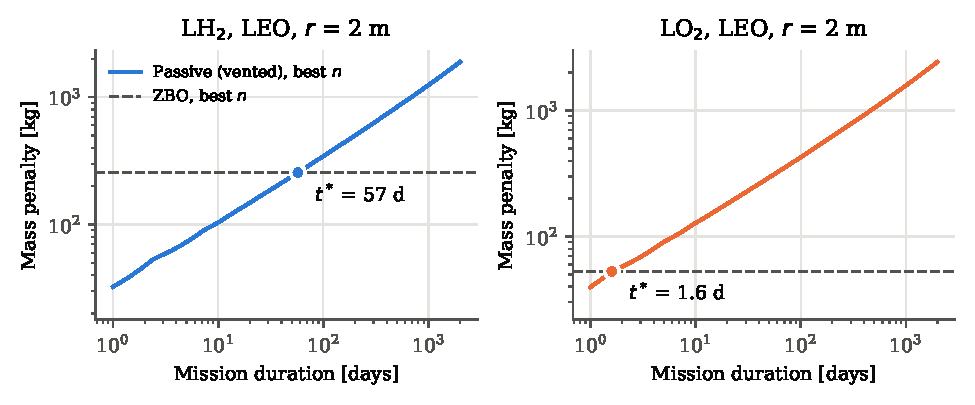
\includegraphics[width=0.8\linewidth]{fig2_mass_vs_duration.pdf}
\vspace{-1.6em}
\caption{Minimum mass penalty against mission duration for the vented passive design and the ZBO design,
each optimised over insulation. The marker is the crossover $t^*$.}
\label{fig:dur}
\end{figure}

\begin{figure}[!htb]
\centering
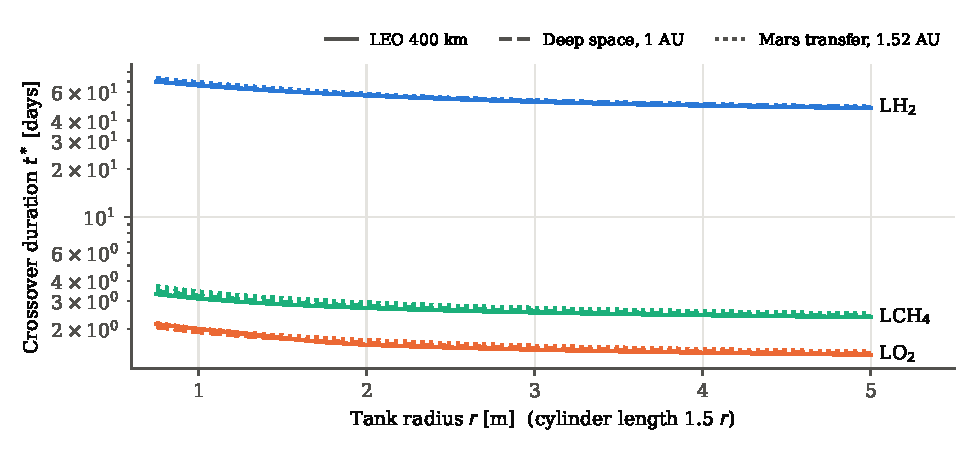
\includegraphics[width=0.72\linewidth]{fig3_crossover_map.pdf}
\vspace{-1.6em}
\caption{First crossover map (vented closure): $t^*$ against tank radius for three propellants and three
environments. The line style marks the environment.}
\label{fig:map}
\end{figure}

\subsection{Closed tank: the ullage closure moves the crossover}
A closed tank absorbs $E_\text{store}$ before its first vent, so for a given insulation choice
$m_\text{lost}=(\Qd_\text{leak}t-E_\text{store})^+/h_{fg}$. Repeating the argument above gives
\begin{equation}
t^*_\text{closed}=t^*_\text{vented}+E_\text{store}/\Qd_\text{leak}=t^*_\text{vented}+t_\text{hold}.
\label{eq:shift}
\end{equation}
Eq.~\eqref{eq:shift} turns objective~R into a direct comparison: \emph{the ullage assumption matters exactly
when the spread in hold time between the two bounds is comparable to $t^*$.} Figure~\ref{fig:hold} and
Table~\ref{tab:closed} evaluate this for venting at 3~bar, with both closures computed exactly from CoolProp.
The homogeneous bound gives hold times of $\thomH$~days (LH$_2$) and $\thomO$~days (LO$_2$). Both are longer
than the vented $t^*$. A thin layer ($m_\text{surf}/m_l=10^{-3}$) holds for only $\thsH$ and $\thsO$~days. A
conduction-only interface layer (\S5, item 1) gives $\tcondH$ and $\tcondO$~days. The resulting crossover spans
$\tcvH$--$\tchH$~days for LH$_2$ and $\tcvO$--$\tchO$~days for LO$_2$: a factor of about 7 for LH$_2$ and several
hundred for LO$_2$. Even the physically anchored conduction layer moves the LH$_2$ crossover from $\tcvH$ to
$\tccH$~days. \emph{First answer to objective~R: the well-mixed assumption moves the crossover, not only the
vent schedule.} Where real tanks sit inside the band is what the spring work refines. Below
$m_\text{surf}/m_l\approx\fdryH$ (LH$_2$) and $\fdryO$ (LO$_2$) the layer evaporates completely before 3~bar
(dotted in Fig.~\ref{fig:hold}); condensation back onto the cold liquid is neglected there, which only
speeds up the pressure rise, so the curve remains a valid fast bound.

\begin{figure}[!htb]
\centering
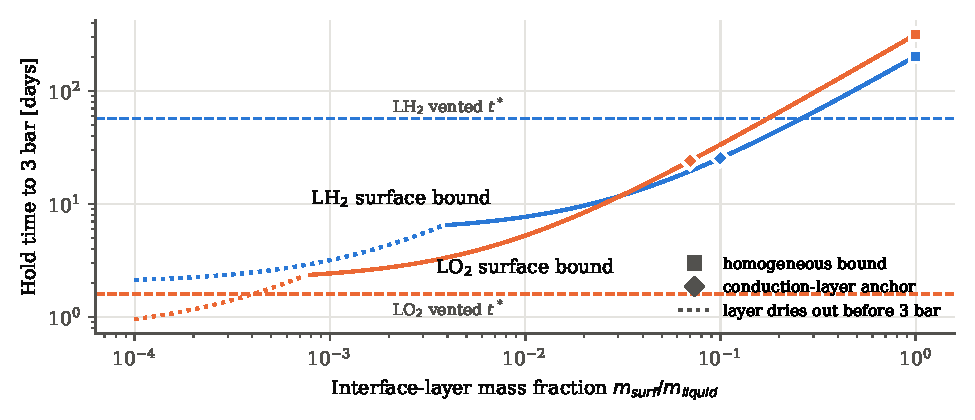
\includegraphics[width=0.78\linewidth]{fig4_hold_time_band.pdf}
\vspace{-1.6em}
\caption{Hold time to 3~bar against interface-layer mass fraction $m_\text{surf}/m_l$ (two-zone surface
bound), with the homogeneous bound (squares, reached exactly at $m_\text{surf}/m_l=1$), the conduction-layer
anchor (diamonds) and the vented $t^*$ (dashed). Dotted: the layer dries out before 3~bar. CoolProp properties.}
\label{fig:hold}
\end{figure}

\begin{table}[!htb]
\centering\small
\caption{Crossover $t^*$ [days] under each closure (LEO, $r=2$~m, 90\% fill, vent at 3~bar). CoolProp properties.}
\label{tab:closed}
\begin{tabular}{@{}lcccc@{}}
\toprule
 & Vented & Surface, $m_\text{surf}/m_l=10^{-3}$ & Surface, conduction anchor & Homogeneous\\
\midrule
LH$_2$ & \tcvH & \tcsH & \tccH\ ($m_\text{surf}/m_l=\fcondH$) & \tchH\\
LO$_2$ & \tcvO & \tcsO & \tccO\ ($m_\text{surf}/m_l=\fcondO$) & \tchO\\
\bottomrule
\end{tabular}
\end{table}

%=====================================================================
\section{Issues identified}
\begin{enumerate}
\item \textbf{$m_\text{surf}$ needs a physical anchor.} As $m_\text{surf}\to0$ the surface-bound hold time
falls to that of the ullage vapour alone (1--2~days here, Fig.~\ref{fig:hold}), so a sweep alone cannot rule
out any answer. A reference scale comes from constant-flux
conduction into a semi-infinite liquid~\cite{carslaw}: $\Delta T_s=(2q/k)\sqrt{\alpha t/\pi}$, which gives
$m_\text{eff}=\tfrac12\rho A\sqrt{\pi\alpha t}$. The sweep will be reported around this anchor.
\item \textbf{The textbook surface closure broke the ordering (resolved).} \texttt{test\_bounds\_ordered} was
written before the L3 physics, and it failed on the first CoolProp run. The $c_p$-form surface layer at
$m_\text{surf}=m$ stored 0.4\% (LO$_2$, LCH$_4$) to 4.4\% (LH$_2$) \emph{more} energy than the homogeneous
bound at 90\% fill, and 30\% less at 30\% fill, so it neither ordered nor collapsed. The cause: it follows
liquid $c_p$ along the saturation line and ignores the vapour. In a nearly full tank the swelling liquid
compresses and condenses the ullage, which releases latent heat, so the constant-volume path needs less
outside energy. The two-zone form (\S2, L3) applies the exact $(\rho,u)$ closure to the warm zone, so
collapse holds by construction and ordering is verified for every $m_\text{surf}/m_l$ from $10^{-4}$ to 1. The
old form is kept in the code as a regression test that records the failure.
\item \textbf{Fill fraction limits the pressure band.} At 90\% fill LH$_2$ is already 98\% liquid by volume
when it reaches 3~bar. At 95\% fill all three propellants become liquid-full first, and the vent pressure is
then reached hydraulically. The model now raises an error in that case rather than returning a subcooled
state; admissible fill will be a trade variable.
\item \textbf{Constant $k_\text{eff}$ and placeholder specific masses} (power, radiator, struts) dominate the
uncertainty in the absolute $t^*$; all are flagged in Table~\ref{tab:params}.
\end{enumerate}

%=====================================================================
\section{Parameter register (Stage 1, in progress)}
\begin{table}[!htb]
\centering\small
\caption{Parameter register. P = provisional (must be sourced before publication); S = sourced.}
\label{tab:params}
\begin{tabular}{@{}p{5.1cm}p{5.6cm}p{4.3cm}@{}}
\toprule
Quantity & Value & Source / status\\
\midrule
$T_\text{sat},\ \rho_l,\ h_{fg}$ (LH$_2$/LO$_2$/LCH$_4$, 1 atm) & 20.3/90.2/111.7 K; 70.8/1141/422 kg/m$^3$; 446/213/511 kJ/kg & S (CoolProp~\cite{coolprop})\\
Cooler mass & $0.2\,\Qd^{0.7}[(T_h-T_c)/T_c]^{1.45}$ kg & S~\cite{plachta2003}\\
Fraction of Carnot $\eta$ & 0.075 (LH$_2$); 0.20 (LO$_2$, LCH$_4$) & P\\
MLI areal density & 0.02 kg/m$^2$ per layer & S~\cite{plachta2003}\\
MLI $k_\text{eff}$, thickness & $3\times10^{-5}$ W/m$\cdot$K; 25 mm per 30 layers & P\\
Outer cover $\alpha/\varepsilon$ & 0.32/0.86 & P (confirm in~\cite{gilmore})\\
Power system; radiator & 0.025 kg/W; 5 kg/m$^2$, $\varepsilon=0.9$, 300 K & P\\
Strut conductance & $5\times10^{-3}$ W/K & P\\
\bottomrule
\end{tabular}
\end{table}

%=====================================================================
\section{Plan to the December milestone}
\begin{enumerate}
\item \textbf{Done (September):} CoolProp test suite run; bounds reformulated, ordering and collapse
verified; all report numbers regenerated from CoolProp.
\item \textbf{Oct, week 1:} Sweep the closed-tank crossover across radius, environment and fill (Fig.~\ref{fig:map}
under all three closures); unify the cooler-mass model between the steady driver and the trade.
\item \textbf{October:} Complete the register (power and radiator specific mass, strut $\int k\,dT$ for G-10 and Ti,
MLI $k_\text{eff}(T)$), and reconcile the LO$_2$ crossover with~\cite{plachta2003}.
\item \textbf{October--November:} Port the 2-D solver to L2 (axisymmetric geometry, radiative boundary
condition via $h_r=\varepsilon\sigma(T^2+T_\infty^2)(T+T_\infty)$); add fill fraction and vent pressure to the trade.
\item \textbf{November:} Validate against published demonstration-tank boil-off (MHTB~\cite{hastings}) to 10\%;
check energy closure below 0.5\%.
\item \textbf{December:} Crossover maps under all three closures; Streamlit interface; public release.
\end{enumerate}
\textbf{Risk:} $t^*$ depends strongly on cooler specific mass, so every map will be published with its
sensitivity to $s_\text{cool}$, $\eta$ and $s_\text{rad}$.

\begin{thebibliography}{9}\footnotesize
\setlength{\itemsep}{0pt}
\bibitem{plachta2003} D.~Plachta and P.~Kittel, ``An updated zero boil-off cryogenic propellant storage analysis
applied to upper stages or depots in an LEO environment,'' NASA/TM, NTRS 20030067928, 2003.
\bibitem{coolprop} I.~H. Bell, J.~Wronski, S.~Quoilin, V.~Lemort, ``Pure and pseudo-pure fluid thermophysical
property evaluation and the open-source thermophysical property library CoolProp,'' \emph{Ind.\ Eng.\ Chem.\ Res.}
53(6):2498--2508, 2014.
\bibitem{zumbo} Zumbo, Ferrero, Masseni, Pastrone, ``Comparison of thermodynamic modelling methods for cryogenic
storage systems,'' AIAA SciTech Forum, 2025.
\bibitem{hastings} L.~J. Hastings et al., Multipurpose Hydrogen Test Bed (MHTB) MLI and boil-off test reports, NASA
MSFC (to be finalised in the register).
\bibitem{gilmore} D.~G. Gilmore (ed.), \emph{Spacecraft Thermal Control Handbook}, Vol.~I, 2nd ed., Aerospace
Press, 2002.
\bibitem{carslaw} H.~S. Carslaw and J.~C. Jaeger, \emph{Conduction of Heat in Solids}, 2nd ed., Oxford, 1959.
\end{thebibliography}
\end{document}
